\documentclass[a4paper,10pt,twocolumn]{article}
\usepackage{txfonts}
\usepackage[utf8]{inputenc}
\usepackage[cyr]{aeguill}
\usepackage{algorithmic, algorithm}
\usepackage{graphicx}
\usepackage{url}
\urlstyle{sf}

%opening
\title{Creating transparent, steerable recommendations}
\author{
Fran\c{c}ois Maillet\\
Sun Microsystems Inc.\\
University of Montreal\\
\texttt{mailletf@iro.umontreal.ca}
\and 
Paul Lamere \\
Sun Microsystems Inc.\\
\texttt{paul.lamere@sun.com}
}
\date{September 2008}

\begin{document}

\maketitle

\begin{abstract}

Music recommendation systems are increasingly important in the ever 
    growing world of digital music.  However, most commercial music 
    recommenders rely on collaborative filtering techniques to generate 
    music recommendations. These type of recommendations lack two aspects 
    that are important for recommendation.  First, they lack transparency 
    - they cannot explain why an item was recommended beyond the trivial 
    ``Other people who listed to XX also listened to YY". Second, they 
    lack steerability - there is no way for a user to interact with the 
    recommender to steer it to more relevant content.
    
    In this demonstration we show the Sun Labs Music Explaura - a 
    web-based recommender that provides transparent and steerable 
    recommendations. The Music Explaura can offer a detailed explanation 
    about why a particular item was recommended and will allow a user to 
    steer the recommendations based upon attributes of the music.

\end{abstract}

\section{The Aura}

In our system for recommending items, each item is
described by a set of words (tags).  These
descriptive words may come from text mining the
web, social annotations, autotagging based upon
content analysis, expert annotation, etc. In our current 
implementation, the most important source for tags 
is the social music website Last.fm, mined using the
Audioscrobbler web services\footnote{Last.fm's Audioscrobbler web services described at http://www.audioscrobbler.net/data/webservices/.}.

The tags provided by Last.fm are weighted by their frequency 
of application. This weighting does not  XXX as a tag like \textit{rock} 
will be applied a large number of times to a large number of bands. 
We hence reweigh the tags based upon their descriptive
content - more descriptive words are given more
weight - using a standard text retrieval weighting function,
TF-IDF. The set of weighted tags for an item is called an
item's `tag cloud", or in a more poetic way, it's aura.

\section{Transparency}

Being able to provide users with transparent recommendations has a lot of advantages. 
For instance, if a user sees a recommendation that makes no sense to him, he might 
lose his trust in the recommender system and stop using it. 

As we represent items in our system using a tag cloud, we determine the similarity 
between two artists as the cosine distance between their respective tag cloud. We chose this 
metric because it implicitly deals the the difference in popularity that exists between artists. 

We are then able to explain why an item is being recommended 
by displaying the overlap between two tag clouds, as shown in figure \ref{fig:commontags}.
Only tags common to the two clouds are displayed and 
their weight is determined by the strenght of the overlap between the tag clouds.

\begin{figure}[ht]
\begin{center}
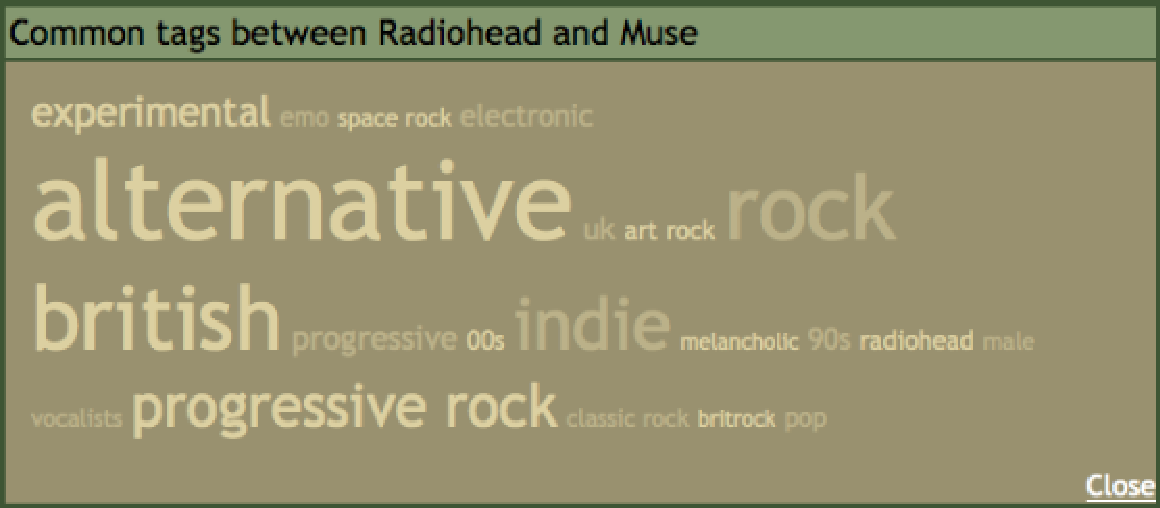
\includegraphics[width=0.9\columnwidth]{radiohead-muse-commontags}
\end{center}
\caption{Common tags between Radiohead and Muse. This tag cloud is displayed as an 
explanation of why Muse is recommended to a Radiohead listener. The tags in the 
clouds are weighted by the strength of the overlap between the two clouds.}
\label{fig:commontags}
\end{figure}

\section{Steerability}
\label{section:steerable}


\begin{figure*}
\begin{center}
\includegraphics[width=0.95\textwidth]{steerable-withtxt}
\end{center}
\caption{The steerable recommendations interface. Users are able to add tags or artists to the cloud by clicking on them from the right hand panel. Then, they can click and drag them to modify their size. A tag that is shrunk below the size of zero will begin to grow again as a negative tag and act as a filter in the returned recommendations.}
\label{fig:steerable}
\end{figure*}

As we provide recommendations to a user, he might dislike them because they are not
based on what he is looking for. For example, he might be looking for a Beatles sounding 
band, but from the 90s, or a Radiohead-like band with a female vocalist. Searching for 
music in this manner is not possible with current recommender systems or any search engine.

By using our patent-pending interface, a user can construct a tag cloud independent 
of any particular item and use this as input to the recommender, as shown in figure \ref{fig:steerable}.
The tag cloud constructed by the user describes the
parameters and concepts that are important to him. The recommender will find items similar to the user's custom
tag cloud in the same way it does it when normally finding similar items.

The user can dynamically and interactively adjust the tag
weights, receiving updated
recommendations in real time after every adjustment. This
allows the user to steer the recommender toward
areas that are of most interest to him. It is possible to shrink some tags to a negative weight to use them as a filter, removing 
any recommended item that contain the negatively weighted tags.

As mentioned earlier, every item in our system is represented by a tag cloud. Even a single tag can be considered as a tag cloud - a tag cloud of only one tag, itself. 
Therefore, any item can be used in a user constructed cloud : a tag, an artist or even another user constructed tag cloud. Users can 
save clouds and reuse them later on, either by themselves or as part of another cloud.

\end{document}
